\documentclass[12pt,a4paper]{report}
\usepackage{graphicx}
\usepackage{subcaption}

\usepackage[utf8]{inputenc}
\usepackage[english]{babel}
\usepackage{caption}
\usepackage{verbatim}
\usepackage{listings}
\usepackage{color}
\usepackage{comment}
\usepackage{pdfpages}
\usepackage{natbib}
\usepackage{booktabs}
\usepackage[toc,page]{appendix}
\usepackage{url}
\usepackage{csvsimple,longtable,booktabs}
\definecolor{codegreen}{rgb}{0,0.6,0}
\definecolor{codegray}{rgb}{0.5,0.5,0.5}
\definecolor{codepurple}{rgb}{0.58,0,0.82}
\definecolor{backcolour}{rgb}{0.95,0.95,0.92}
 
 
 
 \newcommand{\namesigdate}[2][5cm]{%
  \begin{tabular}{@{}p{#1}@{}}
    #2 \\[2\normalbaselineskip] \hrule \\[0pt]
    {\small \textit{Signature}} \\[2\normalbaselineskip] \hrule \\[0pt]
    {\small \textit{Date}}
  \end{tabular}
}
 
 
 
 
 
\lstdefinestyle{mystyle}{
    backgroundcolor=\color{backcolour},   
    commentstyle=\color{codegreen},
    keywordstyle=\color{magenta},
    numberstyle=\tiny\color{codegray},
    stringstyle=\color{codepurple},
    basicstyle=\footnotesize,
    breakatwhitespace=false,         
    breaklines=true,                 
    captionpos=b,                    
    keepspaces=true,                 
    numbers=none,                    
    numbersep=5pt,                  
    showspaces=false,                
    showstringspaces=false,
    showtabs=false,                  
    tabsize=2
}
 
\lstset{style=mystyle}



\graphicspath{ {images/}}
\begin{document}

\begin{titlepage}

\newcommand{\HRule}{\rule{\linewidth}{0.5mm}} 

\center 
 
\textsc{\LARGE University Of Dundee}\\[1.5cm] % Name of your university/college
\textsc{\Large Degree of MSc}\\[0.5cm] % Major heading such as course name
\textsc{\large Data Engineering}\\[0.5cm] % Minor heading such as course title


\begin{figure}
\centering

\includegraphics[width=0.4\textwidth]{dundee.jpg}
\end{figure}

\HRule \\[0.4cm]
{ \huge \bfseries DenseCap}\\[0.4cm] % Title of your document
\HRule \\[1.5cm]
 
\begin{minipage}{0.4\textwidth}
\begin{flushleft} \large
\emph{Author:}\\
Keke \textsc{Zhang} % Your name
\end{flushleft}
\end{minipage}
~
\begin{minipage}{0.4\textwidth}
\begin{flushright} \large
\emph{Supervisor:} \\
Dr. Jianguo \textsc{Zhang}
\end{flushright}
\end{minipage}\\[4cm]

{\large \today}\\[3cm] 


\vfill 

\end{titlepage}
\newpage
\pagenumbering{roman}
\begin{center}
{\huge Executive Summary}
\end{center}
This project refers to Justin Johnson\textsc{\char13}s paper 'DenseCap: Fully Convolutional Localization Networks for Dense Captioning '.This project is based on Convolutional Neural Network(CNN) and Recurrent Neural Network(RNN).The aim of this project is to automatically generate natual language for each salient region accourding to given images.The nerual network model is composed of a Convolutional Neural Network to extract image features, a Fully Convolutional Localization Network to detect objects and a recurrent neural network to general natural language.I evaluate the  network on the subset of Visual Genome dataset,5000 images for testing, 5000 images for evaluateing, and around 40000 images for training.To train the neural network model fast and well, a deep learning framework  Torch and a Titan GPU server were used.
\newpage

\begin{center}
{\huge Declaration}
\end{center}
I declare that the special study described in this dissertation has been carried out and the dissertation composed by me, and that the dissertation has not been accepted in fulfilment of the requirements of any other degree or professional qualification.\\

\vspace{3cm}

\noindent \namesigdate{Name:Keke Zhang}
\newpage


\begin{center}
{\huge Certificate}
\end{center}
I certify that Keke Zhang has satisfied the conditions of the Ordinance and Regulations and is qualified to submit this dissertation in application for the degree of Master of Science.


\vspace{3cm}

\noindent \namesigdate{Name:Dr. Jianguo Zhang}
\newpage

\newpage

\begin{center}
{\huge Acknowledgements}
\end{center}
First of all, I would like to express my sincere thanks to my supervisor, Dr. Jianguo Zhang for his patient and excellent guidance throughout the project.\\
\\
I would also like to thank Professor Annalu Waller and Christopher Norrie for providing the vocabulary list and valuable advice.\\
\\
Last but not least, I would like to thank my parents and friends for their continuous support and understanding.


\newpage
\pagenumbering{arabic}
\section{Introduction}
\subsubsection{Machine Learning}
Machine learning and deep learning has became  more and more popular since the revoluation of dardware.With the development of computation units, for instance GPU (graphics processing unit) and CPU (central processing unit), complicated algorithm and large mounts of computation are  possible.On the other hand, deep learning require huge mounts of traingin data. Nowadays, varieties of web media like Facebook and Youtube make  petabytes of data everyday.This meet the  condition of data volume.Machine learning is a subject that help model   learn exprience. After that, we can use the trained model to predict and make dicisions.

Machine learning could be used in different types of data, images, videos, text, sound et al. In 2017, AlphaGo has won all the three matchs with Ke Jie who was top 1 among all human  go players worldwide.The vectory of AlphaGo not only shows the power of machine learning and also a beautiful future.Machine learning also achieve great success in other field, for instance object detection, speech recognition, face recognition, self-driving et al.
\subsubsection{Revelvent research}
\newpage
\section{Background}
\subsection{Artificial Neural Network}
Artificial neural network is inspired by biological neuron that has input and output.Normally, a typical biological neuron collects  signals in \textit{dentrites} and send out the signal through \textit{axon}.There is a structure called \textit{synapse} between neurons, it decides whether the signal will pass \textit{synapse} and arrive next neuron.
\begin{figure}[h]
\begin{subfigure}{0.5\linewidth}
	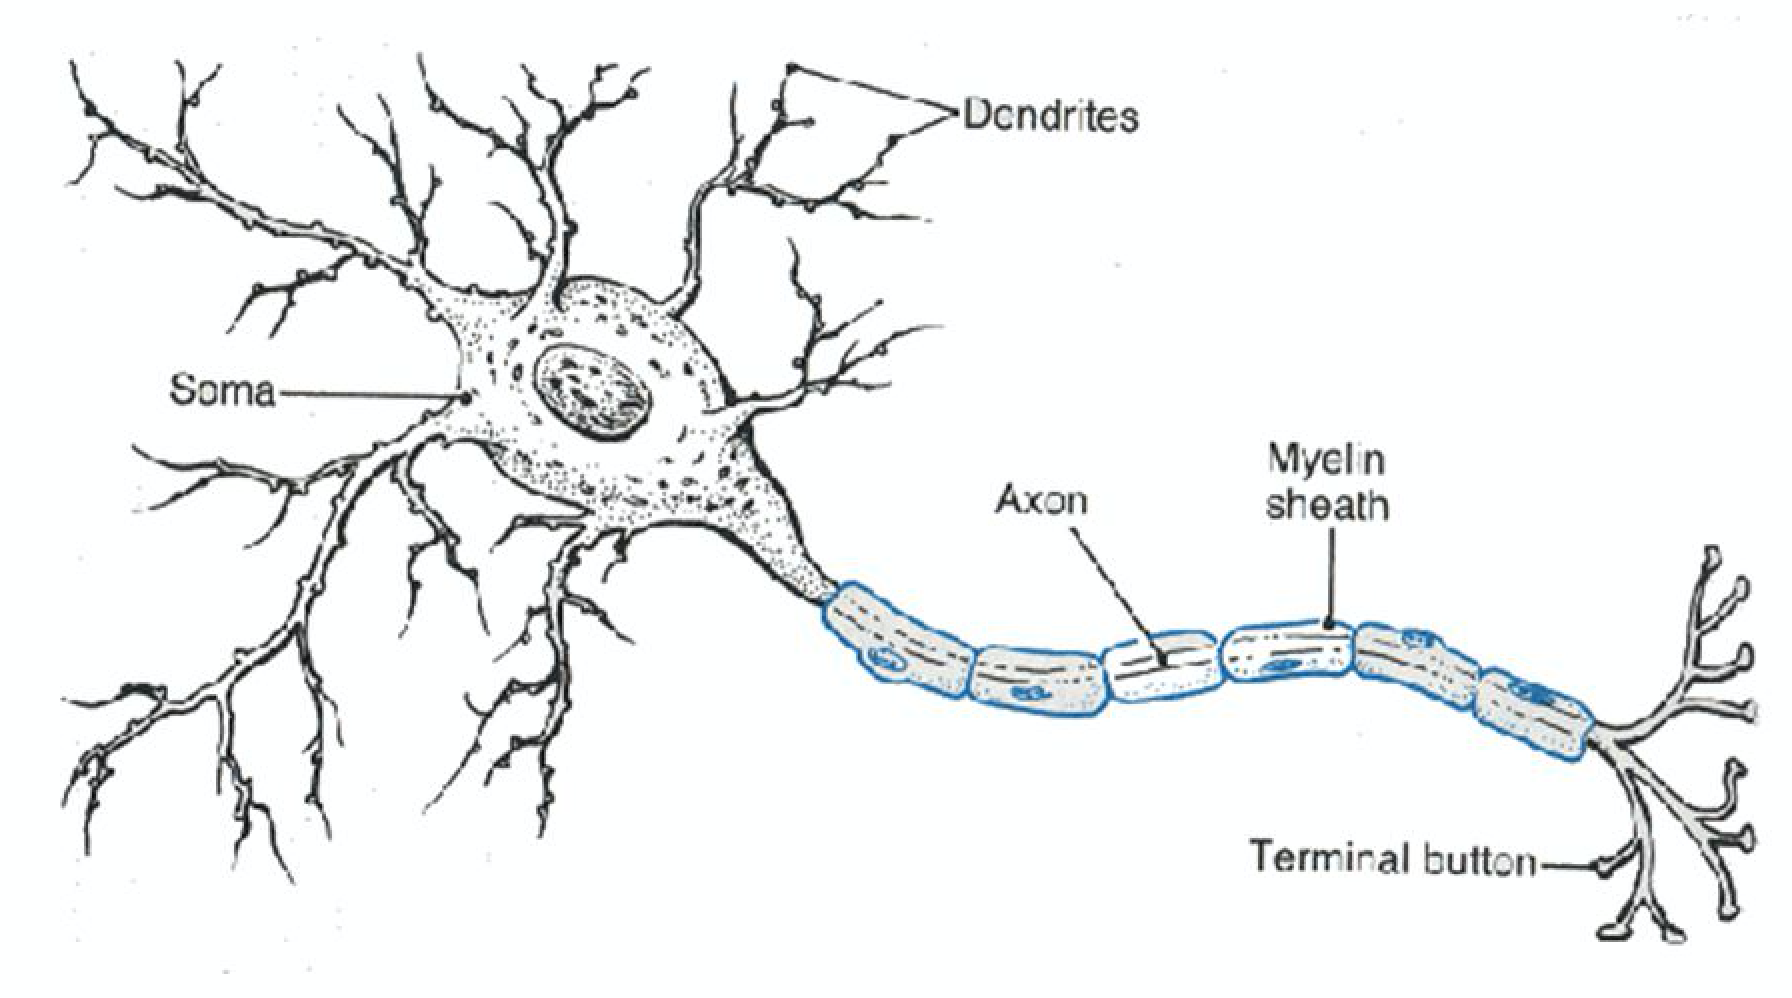
\includegraphics[height=3.5cm,width=\textwidth]{n1.png}
	\caption{Biological Neuron}
\end{subfigure}
\begin{subfigure}{0.5\linewidth}
	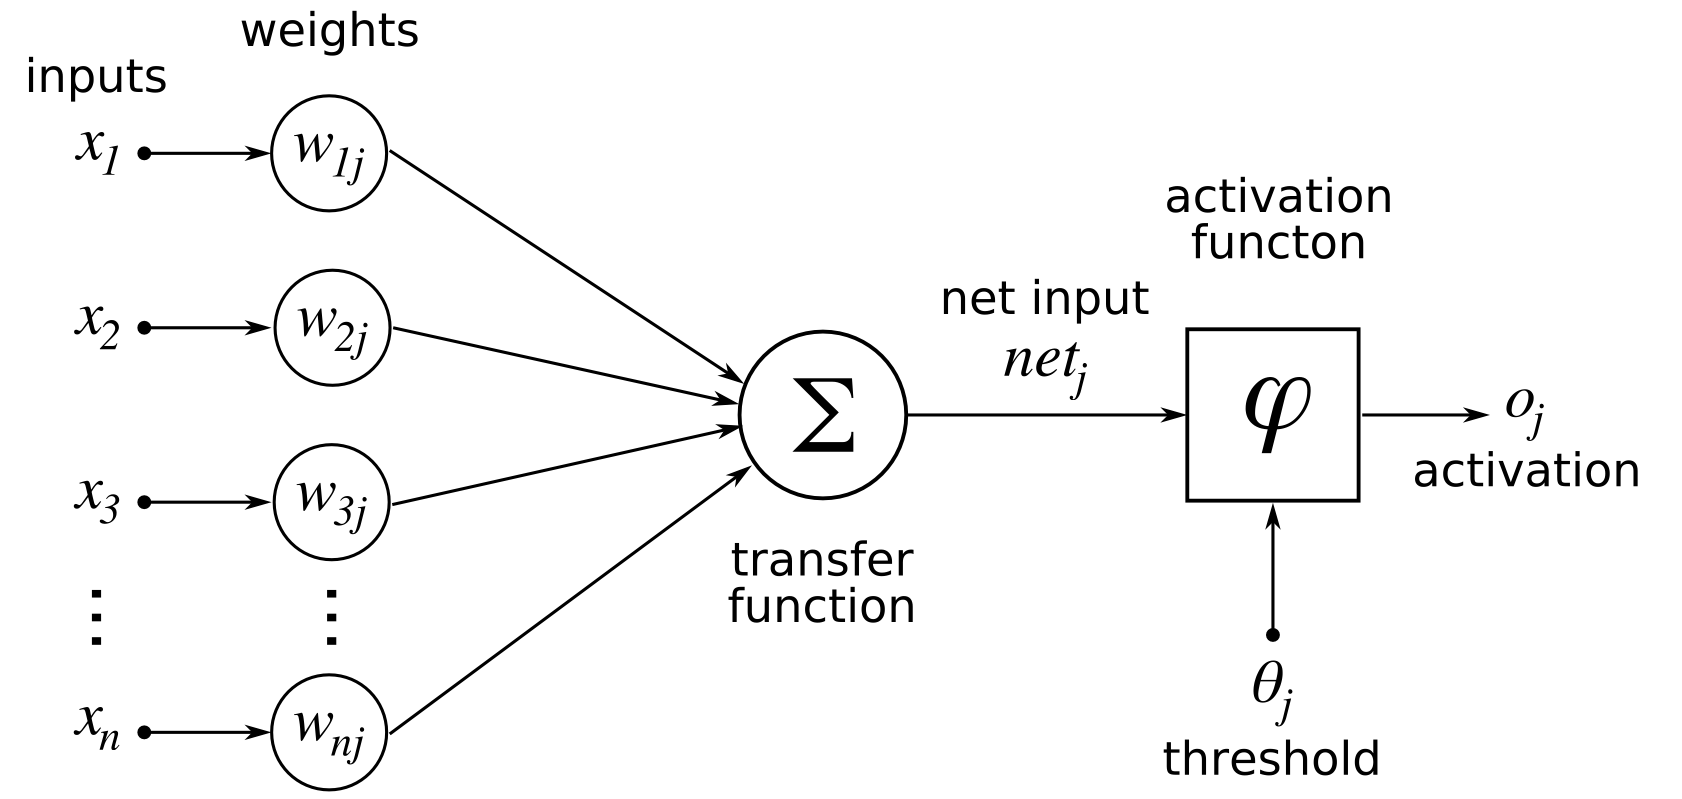
\includegraphics[height=3.5cm,width=\textwidth]{Aneuron.png}
	\caption{Artificial Neuron}
\end{subfigure}
\label{Biological Neuron and Artificial Neuron}
\caption{Biological Neuron and Artificial Neuron}
\end{figure}
An artificial neuron is an information cell which can compute input with some special algorithm and output results.An artificial neural network is composed of hundreds or thousands of neurons.Each neuron gets input from last layer neurons and output to next neurons.The first layer is called input layer, the last layer is output layer, and all layers between the input layer and output layer are the hidden layer.Normally, we consider the Artificial neural network as a black box. It read data in the input layer and output result after amounts of computation.\\

\begin{figure}[h]
\centering
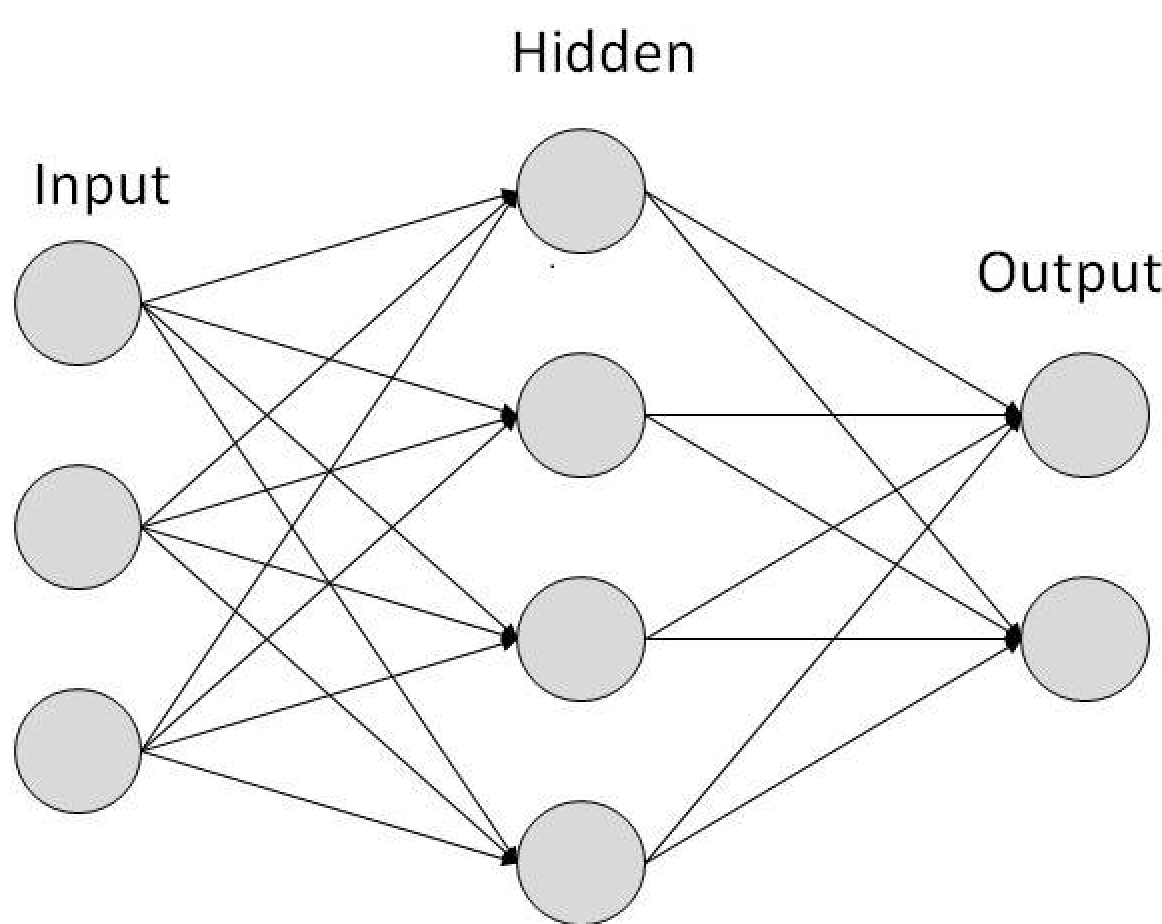
\includegraphics[height=3cm,width=0.4\textwidth]{nn1.png}
\caption{Neuron Network}
\end{figure}

\newpage

Like biological neurons have \textit{synapse}, each artificial neuron has a  computation cell called activation function. The activation function will decides whether and how much the data can output to next neuron.Next figure is showing different types activation function.Unlike biological neurons, artificial neurons also have weights and biases.Before input to activation function all inputs should go through a transfer function unit.\\

Transfer function:

\[z= \sum\limits_{i}W_i X_i +b\]

Activation function:
	\[\phi(z)\]
\begin{figure}[h]
\centering
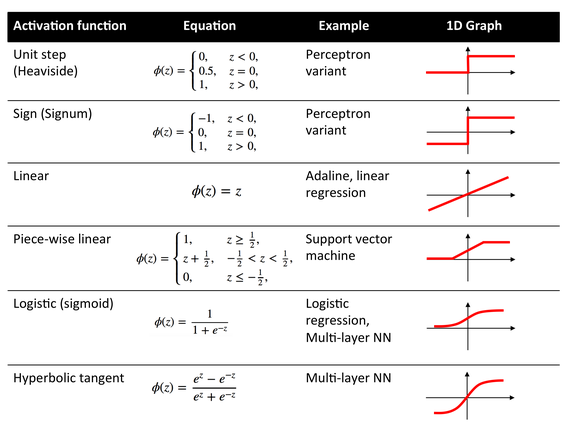
\includegraphics[width=0.9\textwidth]{activation.png}
\caption{Different types activation}
\end{figure}

\newpage

A neural network is not enough to do some real jobs, it only contains initialized parameters.To make it works, we need to train the neural network.Error backpropogation is a powerful weapen in almost all the real life jobs.A training iteration consists two parts, forward propagation and backward propagation(BP). As we mentioned, forward network pass  data from input layer until output layer, while backward pass error from output layer back to input layer.Before we dig deeper in BP, a loss function should be defined in advance. The loss function is a tool to evaluate  the difference (Error) between the output and the target output.In general, all the neural network jobs are always around the error.The goal is to minimize the error, to optimize the network parameters.A practical example is belowing to help understand Backpropagation and Gradient decent.

\textbf{Example for Backpropagation:}
Assume that every day you have lunch at the cafeteria, you diet only consists of fish , chips, and ketchup. The cashier only tells you the total price of the meal. A few days later, you should be able to figure out the single price of each food.

Assume price of means is 850, and use linear activation function and squared error function in this example.\\
Target Price: 850\\
Portions of fish: 2\\
Portions of chips: 5\\
Portions of ketchups:3\\
\[Price=X_{fish} W_{fish}+X_{chips}W_{chips}+X_{ketchup}W_{ketchup}\]
First we star with random guess the prices:
\[W_{fish}=W_{chips}=W_{ketchup}=50\]
$So,price=2\times 50+5\times 50+3\times 50=500$
\[E=\frac{1}{2} \sum\limits_{n\in training}(t^n-y^n)^2\]

\begin{figure}[h]
\centering
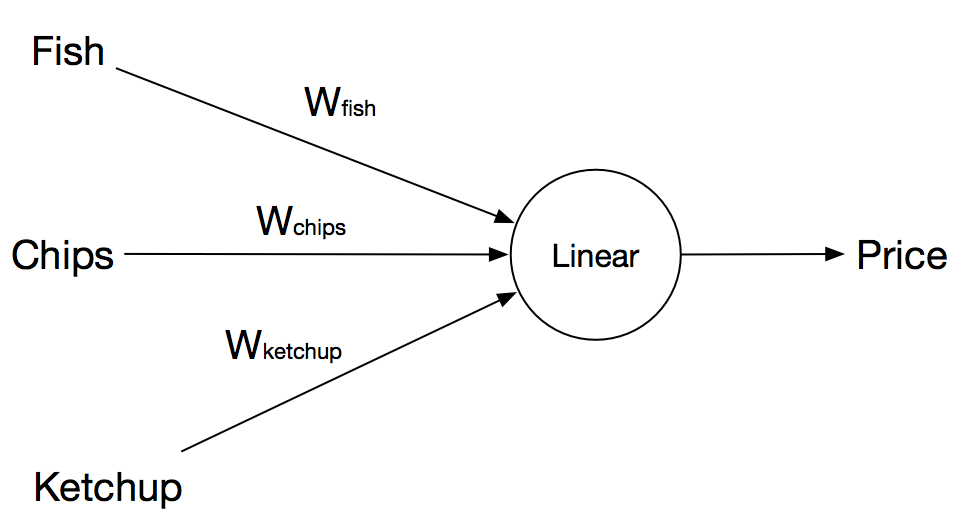
\includegraphics[width=0.5\textwidth]{bp.png}
\caption{BP example }
\end{figure}
\newpage
Where:
$t$ is target price,$y$ is output price, $\varepsilon$ is learning rate(assume 1/35).
\[\frac{\partial{E}}{\partial{w_i}}=\frac{1}{2}\sum\limits_n\frac{\partial{y^n}}{\partial{w_i}}\frac{d{E^n}}{d{y^n}} =-\sum\limits_n x_i^n(t^n-y^n)\]

\[\Delta w_i=-\varepsilon\frac{\partial E}{\partial w_i}=\sum\limits_n \varepsilon x_i^n(t^n-y^n)\]
In this case n=1.\\
Thus $ \Delta w_i =\frac{1}{35}x_i(850-500)$\\

$\Delta w_{fish}=20,\Delta w_{chips}=50,\Delta w_{ketchup}=30$   \\

Update to\\

$w_{fish}=70,w_{chips}=100,w_{ketchup}=80$  \\

$ Price=2\times 70+5\times 100+3\times 80=880$\\
 
One more iteration\\

$\Delta w_{fish}=-1.7,\Delta w_{chips}=-4.3,\Delta w_{ketchup}=-2.6$   \\

Update to\\

$w_{fish}=68.3,w_{chips}=95.7,w_{ketchup}=77.4$  \\

$price=2\times 68+5\times 95.7+3\times 77.4=847.3$\\
As the above computation  shows, total price is 500 , 880 then 847.3.With enough iterations, there is no doubt the total price will converge to 850, the target output.
\subsection{Convolution Neural Network(CNN)}
In image processing and computer vision field, the images are usually  represented as pixel vectors.For instance, there is a 1000 by 1000 image, so this image could be present as a 1000000-dimension vector.If the hidden layer has same number of neurons as input layer. Then the number of weights should equels 1000000*1000000=$10^{12}$. $10^{12}$ weight is too many to be trained.In other words, it is  impossible for hardware to process so many parameters.In order to process images in neural network, we have to reduce parameters.
\subsubsection{Local Connectivity}
In general, The spatial connection of the image is also the local pixel contact is more closely, and the distant pixel correlation is weak.Thus, each neuron is not necessary to perceive the global image, only need to perceive the local, and then at the higher level will be part of the information together to get the overall information.As the instance we mentioned before, assume each neuron only connects to 10*10 neurons, then paremeters will reduce from $10^{12}$ to $10^8$.In fact, it is equivalent to convolution operation.
\begin{figure}[h]
\centering
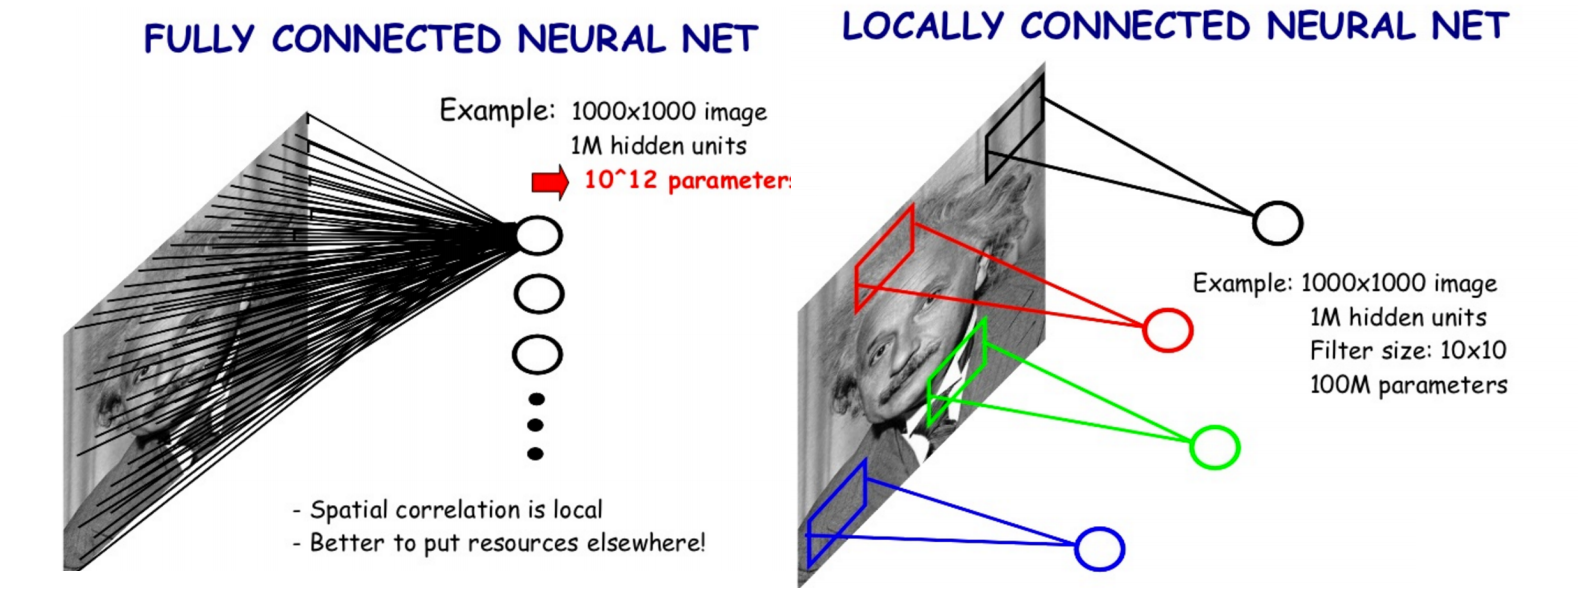
\includegraphics[width=0.9\textwidth]{localconnect.png}
\caption{Fully connected and local connected network}
\end{figure}
\subsubsection{Parameters Sharing}
However,$10^8$ parameters is still too large for a neural network.The other power weapon to reduce parameters is parameter sharing.In the above local connected instance, each neuron corresponds to 100 parameters, there are a total of 1000000 neurons.If  all the 1000000 neurons have the same 100 parameters, then the number of parameters reduce to 100.\\
\begin{figure}[h]
\centering
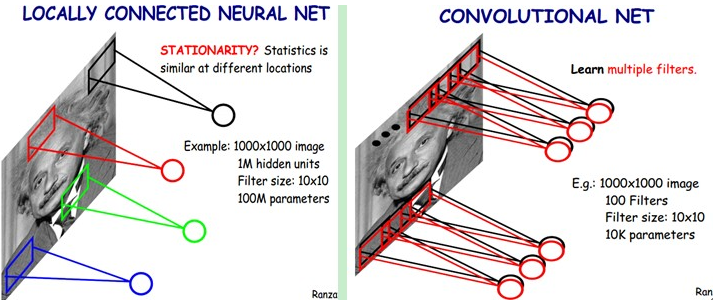
\includegraphics[height=4cm,width=0.9\textwidth]{parameter.png}
\caption{Multiple convolution kernels}
\end{figure}
To understand the weight of sharing better, we consider these 100 parameters (that is, convolution operations) as a way of extracting features that are independent of position. The implication of this is that the statistical properties of a part of the image are the same as those of the other parts. This also means that the features we learn in this part can also be used on another part, so we can use the same learning feature for all the positions on the image.Normally, one feature is not enough for an image, so it is better to use multiple kernel to learn multiple features.
\subsubsection{Convolution Layer}
convolution layer is the core layer of a convolutional neural network, which compute dot product between the filters and the input data. In image processing, input data usually has three dimension, width, height and depth. The convolution kernel depth has to match input volume	depth.In other words, the number of channels have to be same.	Next figure is showing a practical example of what convolution does.	
\begin{figure}[h]
\centering
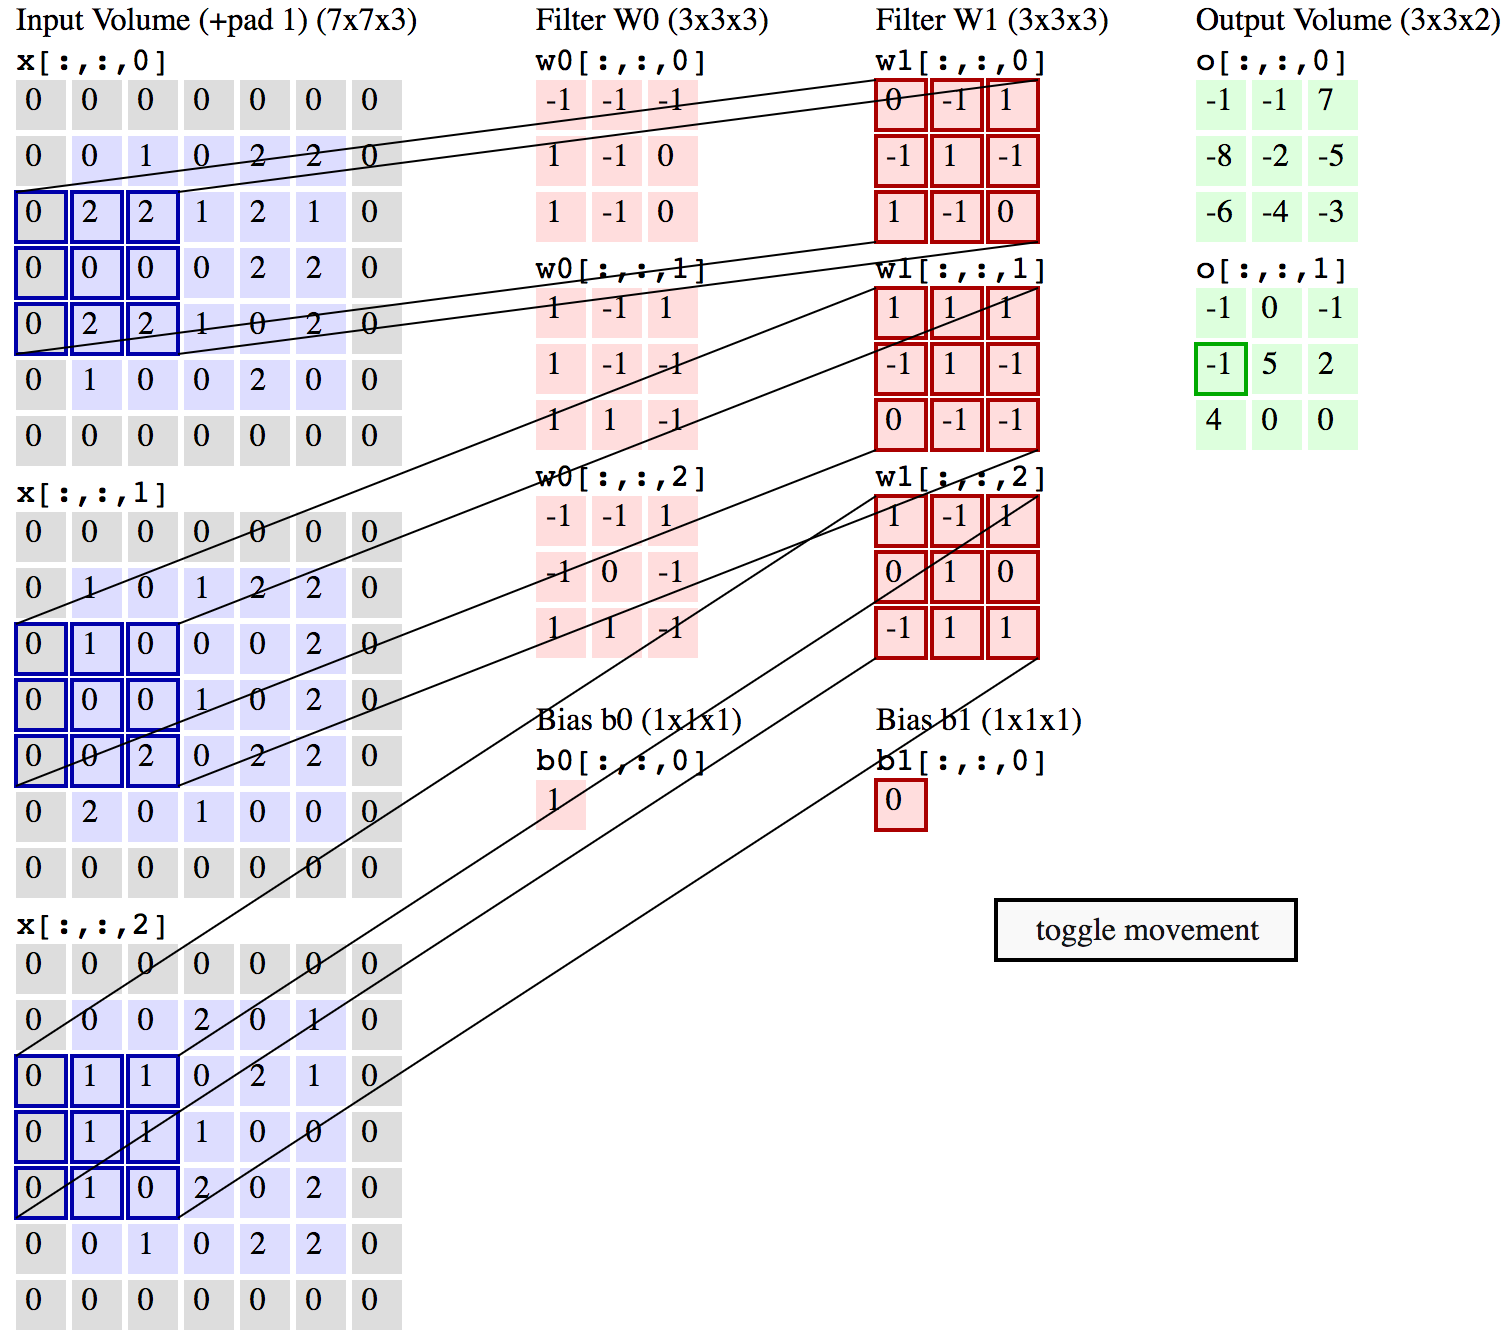
\includegraphics[width=0.9\textwidth]{conv.png}
\caption{Convolution}
\end{figure}

In general, if a convolution layer with:
\begin{itemize}
\item Input vulome with size $W_1\times H_1\times D_1$
\item Number of kernels K
\item Zero padding width P:the gray cell with value 0 in fugure 5, zero padding is only for controling of output shape.
\item The stride S:step size of sliding kernel.
\item Kernel size F
\end{itemize}

Produce a volume of size $W_2 \times H_2 \times D_2$ where:
\begin{itemize}
\item $W_2=(W_1-F+2P)/S+1$
\item $H_2=(H_1-F+2P)/S+1$
\item $D_2=K$
\end{itemize}

The input volume size is 5x5x3,zero padding size 2, with two 3x3x3 kernels.
\begin{itemize}
\item $W_2=(5-3+2 \times 1)/2+1=3$
\item $H_2=(5-3+2 \times 1)/2+1=3$
\item $D_2=2$
\end{itemize}
With the equation we can easily compute output volume shape 3x3x2.

\newpage
\subsubsection{Pooling Layer}
After convolution layer, the next step is to use these features to do the classification jobs. Theoretically, we can use all the extracted features to train the classifier, such as the softmax classifier, but this is facing with the challenge of calculating the amounts of computation and overfitting.A pooling layer is usually followed a convolution layer to control overfitting and spatial size of data.The most common form is a pooling layer with 2x2 size kernels which match the depth to input volume.At most of time, the kernel with a stride of 2.Assume a Max poling is applied, that means the operation will pick the maximum value from every possible  2x2 region.

\begin{figure}[h]
\centering
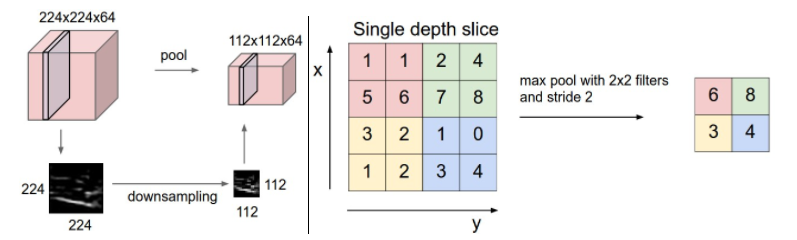
\includegraphics[width=0.9\textwidth]{pooling.png}
\caption{Pooling operation}
\end{figure}
In summary, a pooling layer with:
\begin{itemize} 
\item input volume $W_1 \times H_1 \times D_1$
\item filter size F
\item stride S

Produces an output volume$W_2 \times H_2 \times D_2$, where:
\item $W_2=(W_1-F)/S+1$
\item $H_2=(H_1-F)/S+1$
\item $D_2=D_1$
\end{itemize}

\newpage

\subsubsection{Some Popular CNN Architectures}
\begin{itemize}
\item \textbf{LeNet:} First successful CNN Architecture which developed by Yann LeCun in 90s.
\begin{figure}[h]
\centering
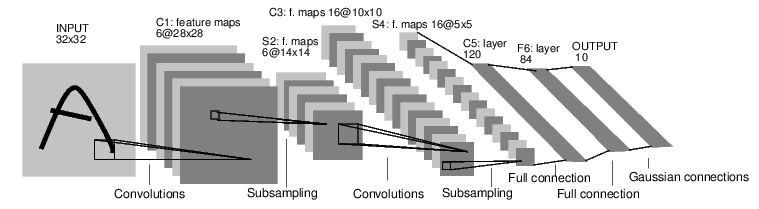
\includegraphics[width=0.8\textwidth]{lenet.png}
\caption{LeNet Architecture}
\end{figure}
\item \textbf{AlexNet:} AlexNet was developed by Alex Krizhevsky, Ilya Sutskever and Geoff Hinton. The AlexNet achieved second runner-up in ImageNet ILSVRC challenge in 2012.It was  very similar to LeNet, but bigger and deeper than it.
\begin{figure}[h]
\centering
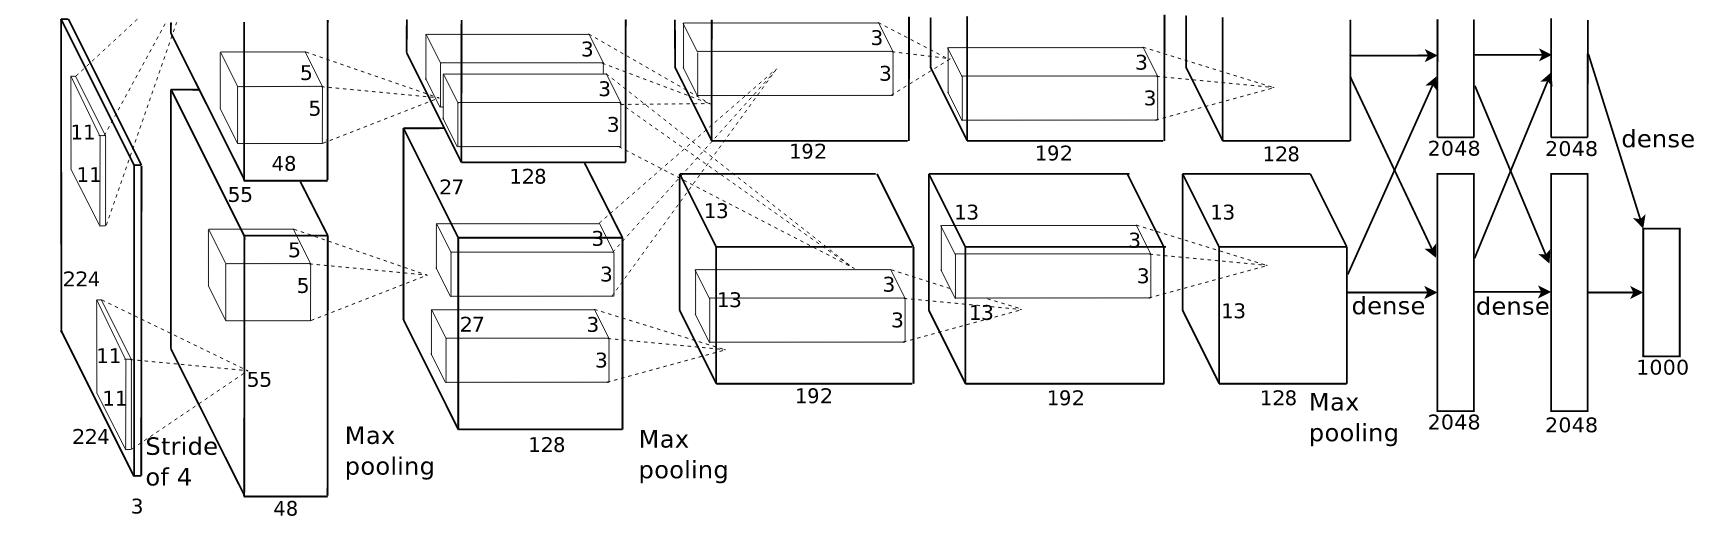
\includegraphics[width=0.8\textwidth]{alexnet.png}
\caption{AlexNet Architecture}
\end{figure}
\item \textbf{ZFNet:} ZFNet was a provement version of AlexNet which came from Matthew Zeiler and Rob Fergus.The CNN architecture also made  them winner in ILSVRC 2013.Compare to AlexNet, ZFNet has bigger size of middle convolution kernel and smaller stride.
\item \textbf{GoogleNet:}  Szegedy et al was the author of GooleNet, and he also won the ILSVRC 2014.GoogleNet reduce a large amount of  parameters from 60M to 4M(compared to AlexNet).
\item \textbf{VGGNet:}VGGNet was runner-up in ILSVRC 2014 which came from Karen Simonyan and Andrew Zisserman.The VGGNet proved that deeper neural network not always have better perfermance.On the other side VGGNet cost a lot of memory for parameters(14M).In this project we use VGG-16 which composed of 13 convolution layers and 3  fully connected layers.



\begin{figure}[h]
\centering
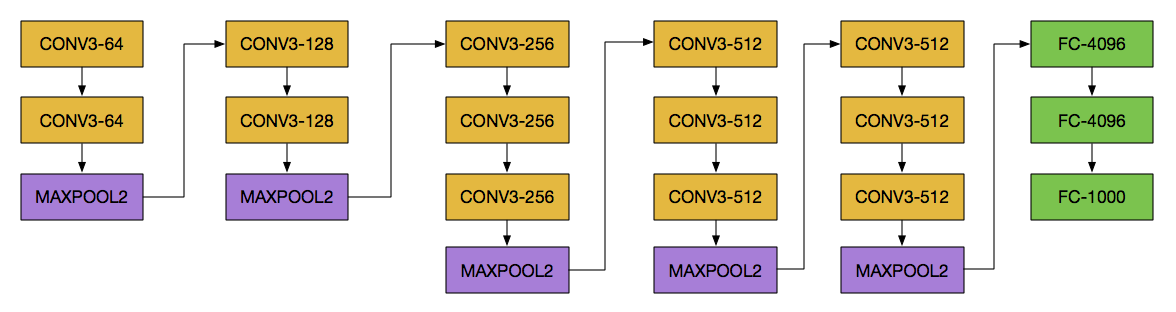
\includegraphics[width=0.9\textwidth]{vgg16.png}
\caption{VGG-16 Architecture}
\end{figure}

\end{itemize}
\newpage
\subsection{Recurrent Neural Network(RNN)}



\section{Requirements Specification}

\section{Design}

\subsection{Platform and dependences}
This project is running on Torch, it is a open source deep learning framework which can build network architecture and train it. It is also a script language based on Lua programming language.It is efficient and easy to use, except it lacks Python Interface.So in this project, some data exchange between Lua script and Python script is on JSON forma.Torch7 is the version using in this project, but Torch is not the only one library.It also requires some other libraries for neural networks, images and GPU computation.

\begin{itemize}
\item nn
\item nngraph
\item image
\item lua-cjson
\item stnbhwd
\item torch-rnn
\end{itemize}
All these common dependences can be easily install by Luarocks.However, network training is very slow in only CPU model, especially for large dataset.To train the network faster,GPU accelerate is a popular strategy.In that case a NVIDIA GPU and CUDA library  are necessary.Then, you will also need  install several libraries on Torch.
\begin{itemize}
\item cutorch
\item cunn
\item cudnn
\end{itemize}
As we mentioned before, Python script  is necessary as well. Python language is foucuing on dataset processing in this project, including editing region relationship JSON file, objects and words extracting, combining images and JSON file into HDF5 format.I am using python 2.7 through all this project and some python modules is also require as well.
\begin{itemize}
\item numpy
\item scipy
\item pillow
\item h5py
\item json
\item random
\item pprint
\end{itemize}
\subsection{Dataset}
This image dataset I am using is Visual Genome Dataset, it contains around 94,000 images and 4,100,000 regions-grounded captions.The whole dataset is too large for my project, i only use a subset of it.The subset dataset is comprises 5000 images for testing, another 5000 images for evaluating, and 40000 images for trining.
This dataset is not only images, it also contains some JSON files which help to allocate objects' coordinate axis, describe regions and objects.Next figure showing image examples and JSON file examples in from the dataset.

\begin{figure}[h]
\centering
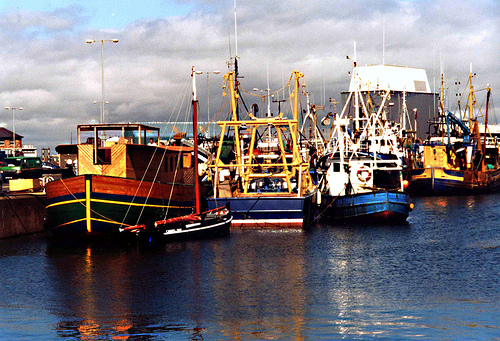
\includegraphics[width=0.8\textwidth]{2356274.jpg}
\caption{Imges Example}

\end{figure}
\newpage

\begin{figure}[h]
\begin{subfigure}{0.5\linewidth}
	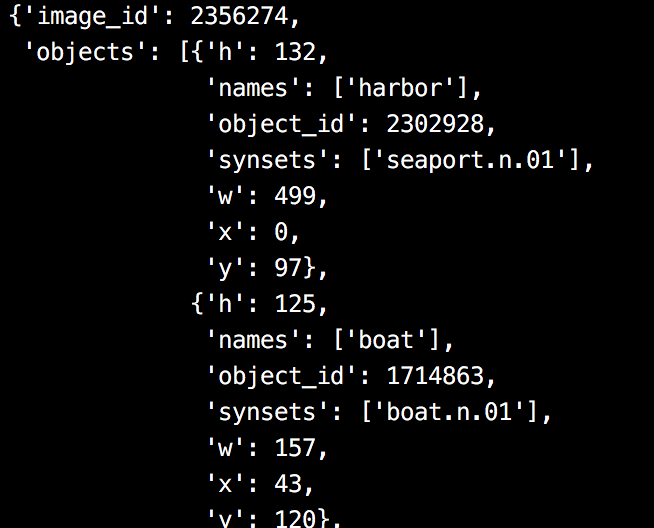
\includegraphics[height=5.5cm,width=\textwidth]{object.png}
	\caption{Object Example}
\end{subfigure}
\begin{subfigure}{0.5\linewidth}
	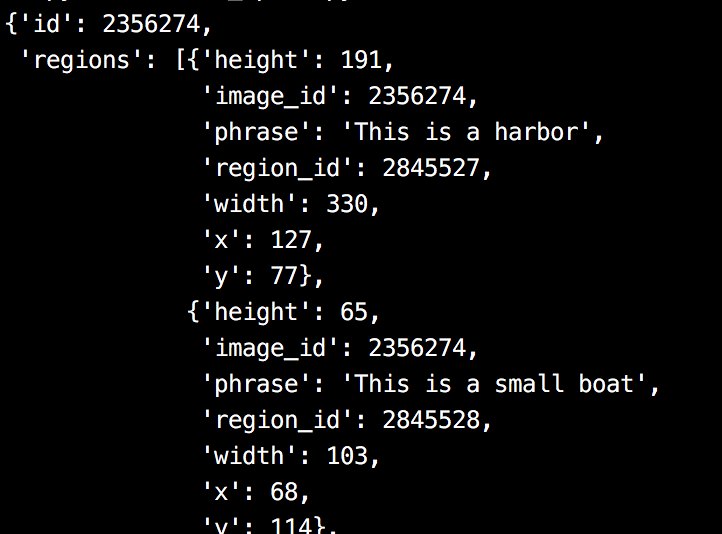
\includegraphics[height=5.5cm,width=\textwidth]{region.png}
	\caption{Region Description Example}
\end{subfigure}
\label{dataset example}
\caption{JSON File Example}
\end{figure}

As for vocabulary dataset, it comes from University of Aberdeen.Thanks to Professor Annalu Waller and Christopher Norrie, they have chosen the most valuable 166  words for this project. All these 166 words form the whole vocabulary.

\begin{figure}[h]
\centering
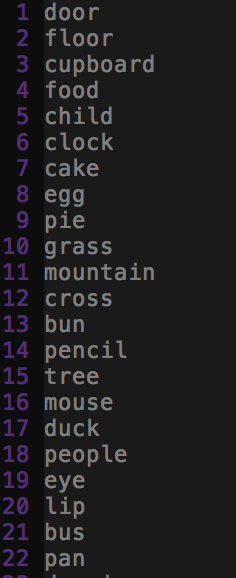
\includegraphics[width=0.2\textwidth]{vocab.png}
\caption{Vocabulary Example}
\end{figure}

Neural networks can not read images and vocabulary directly, all data must convert to HDF5 format.First of all, remove all images which their region phrase do not included in vocabulary list.Then randomly assign these images into train set, test set and evaluate set.(5000 images in test set and 5000 images in evaluate set, others remain to training set.)
\subsection{TO BE continue}


\newpage
\subsection{Networks}
\subsubsection{VGG-16}
The whole project composed of three main neural networks,VGG-16(Convoluational Neural Network), Object detection and Recognition Network  and Recurrent Neural Network language model.

\begin{figure}[h]
\centering
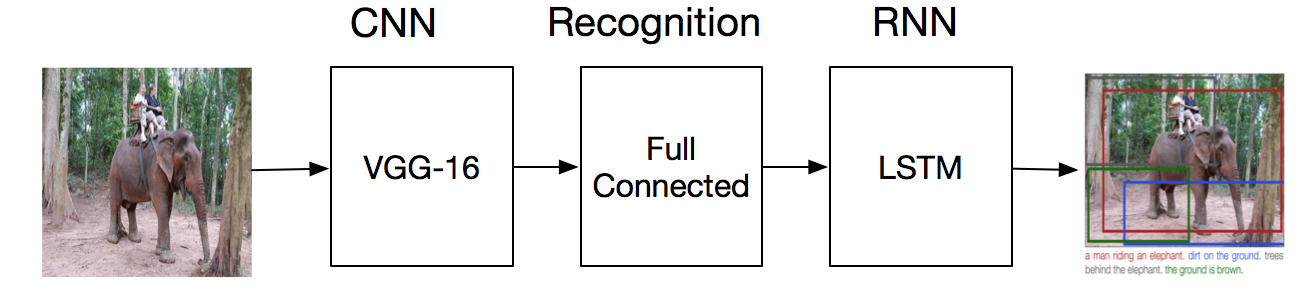
\includegraphics[width=0.9\textwidth]{network.png}
\caption{Main networks}
\end{figure}
At the begining of the neural network, a VGG-16 was used to extract features.And this VGG-16 has been pretrained by ImageNet.\\

(NEED TO ADD VGG details)\\
As we mentioned before, The VGG-16 architecture composed of 13 layers of  3$\times $3 convolution kernels and 5 layers of 2$\times$2 max pooling kernels.In this project we only remain the first four max pooling layers.

\begin{figure}[h]
\centering
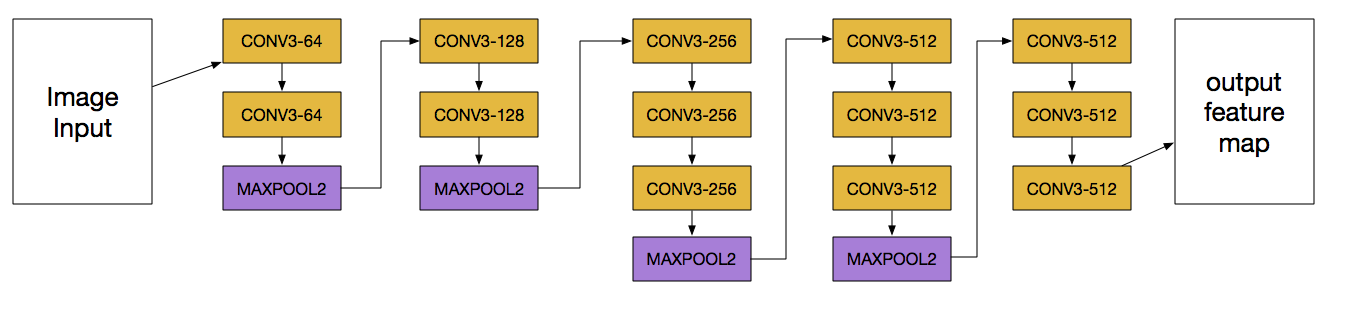
\includegraphics[width=0.9\textwidth]{vgg162.png}
\caption{VGG-16 Architecture}
\end{figure}

Assume that we feed the network a images size of 3$\times$224$\times$224. \\
In summary :
\begin{itemize}
\item input volume 3$\times$224$\times$224
\item filter size 3$\times$3
\item stride 1
\item zero padding 1
\end{itemize}

width=(224 - 3+2$\times$1)/1+1=224, height=(224 - 3+2$\times$1)/1+1=224\\
So for each time the image go through convolution layer width and height remains the same. As for pooling layer, each 2$\times$2 pooling will reduce the tensor size to a half.We have 4 layers of max pooling, so $width=224/2^4=14$,$height=224/2^4=14$.In a word, the VGG-16 will convert a 3$\times$224$\times$224 RGB image to a 512$\times$14$\times$14 tensor.(We use 512 kernels in last convolution layer).The output of this VGG-16 neural network will feed to region proposal network(RPN) in next main neural network.
\subsubsection{Fully Convolutional Localization Network(FCLN)}
A Region Proposal Network(RPN) takes feature maps as input from last networks(In my case it is VGG-16 as we mentioned before) and outputs a set of proposal regions which has been marked with  scores.
To general region proposals, we use a sliding-window through the convolutional feature maps.Each sliding-window can general k anchors.We use 3 scales and 3 aspect ratios for each sliding-window, so $k=3\times 3=9$.And all these 9 anchors are centered at the same sliding-window.

\begin{figure}[h]
\centering
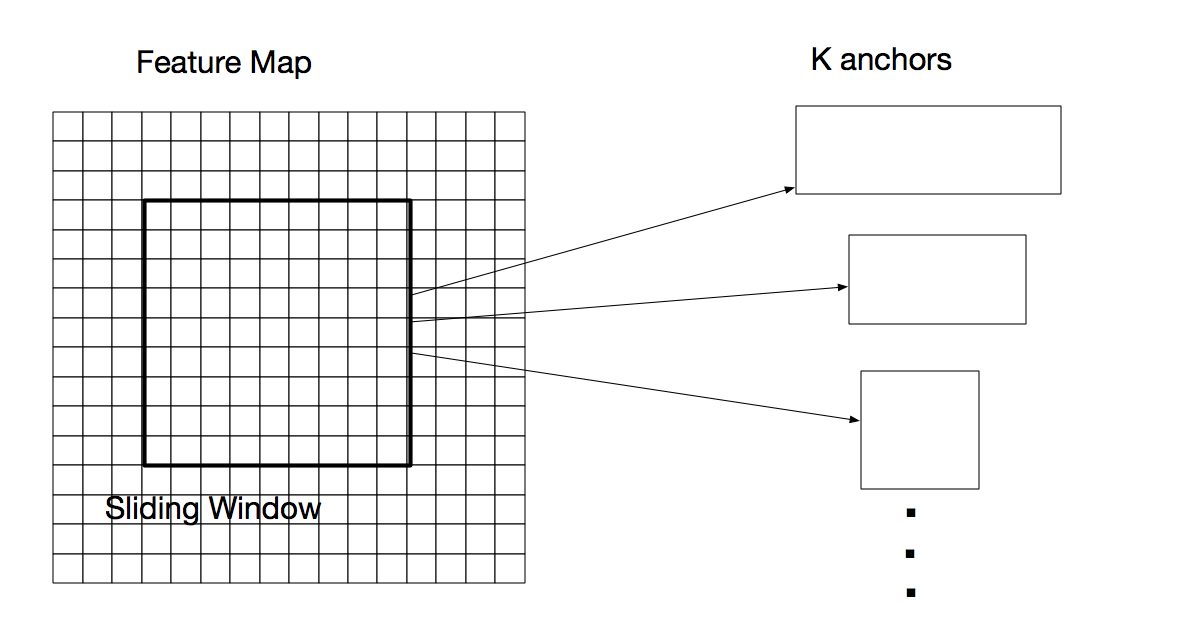
\includegraphics[width=0.9\textwidth]{sliding.png}
\caption{Generating anchors}
\end{figure}

For each of these k anchors, we predict a score and four scalar regressing from anchor to region coordinates.
To do these, we feed our feature map to a $3\times 3$ convolution with 256 kernels, then through  a rectified linear nonlinearity, and a $1\times 1$ convolution with 5k kernels.The output is a $5k\times W'\times H'$ tensor which contains  all scores and scalars regresses.
\newpage
\begin{figure}[h]
\centering
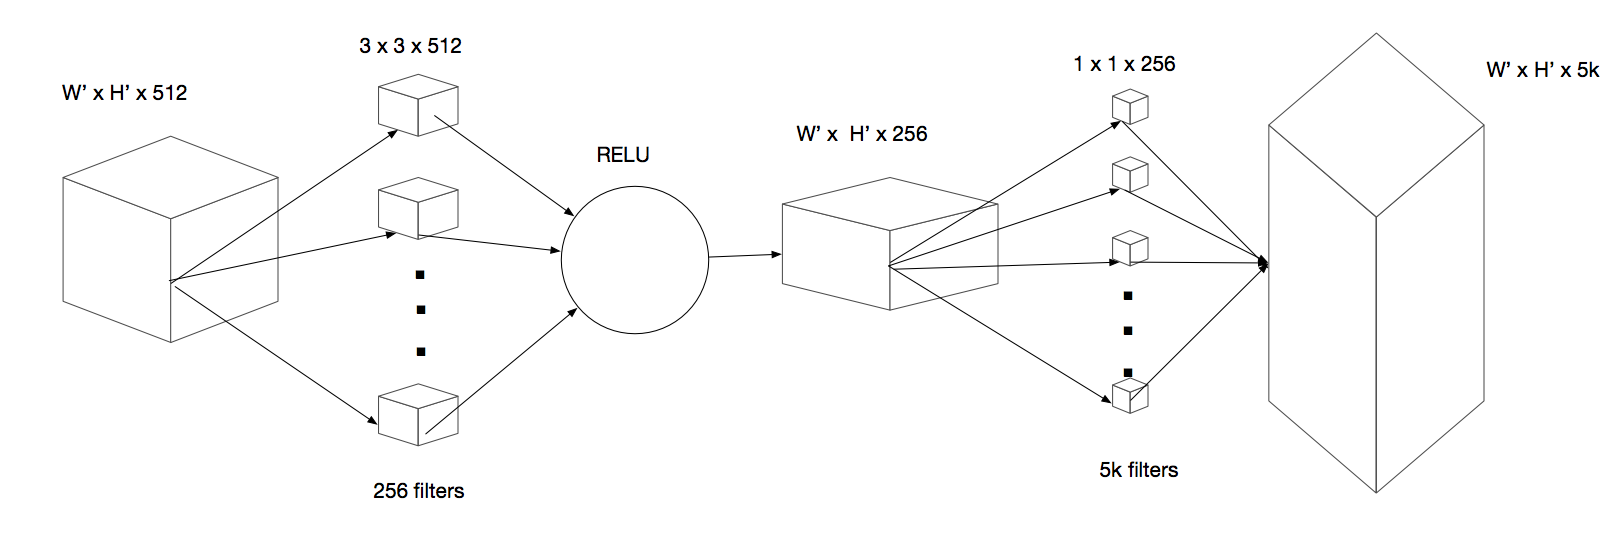
\includegraphics[width=0.9\textwidth]{computeanchors.png}
\caption{Coompute anchors}
\end{figure}

Given an anchor with center $(x_a,y_a)$, width $w_a$,height $h_a$, scalas as we computed before$(t_x,t_y,t_w,t_h)$will project anchor coordinates to original region coordinates.
\[x=x_a+t_xw_a\]
\[y=y_a+t_yh_a\]
\[w=w_aexp(t_w)\]
\[h=h_aexp(t_h)\]


\begin{figure}[h]
\centering
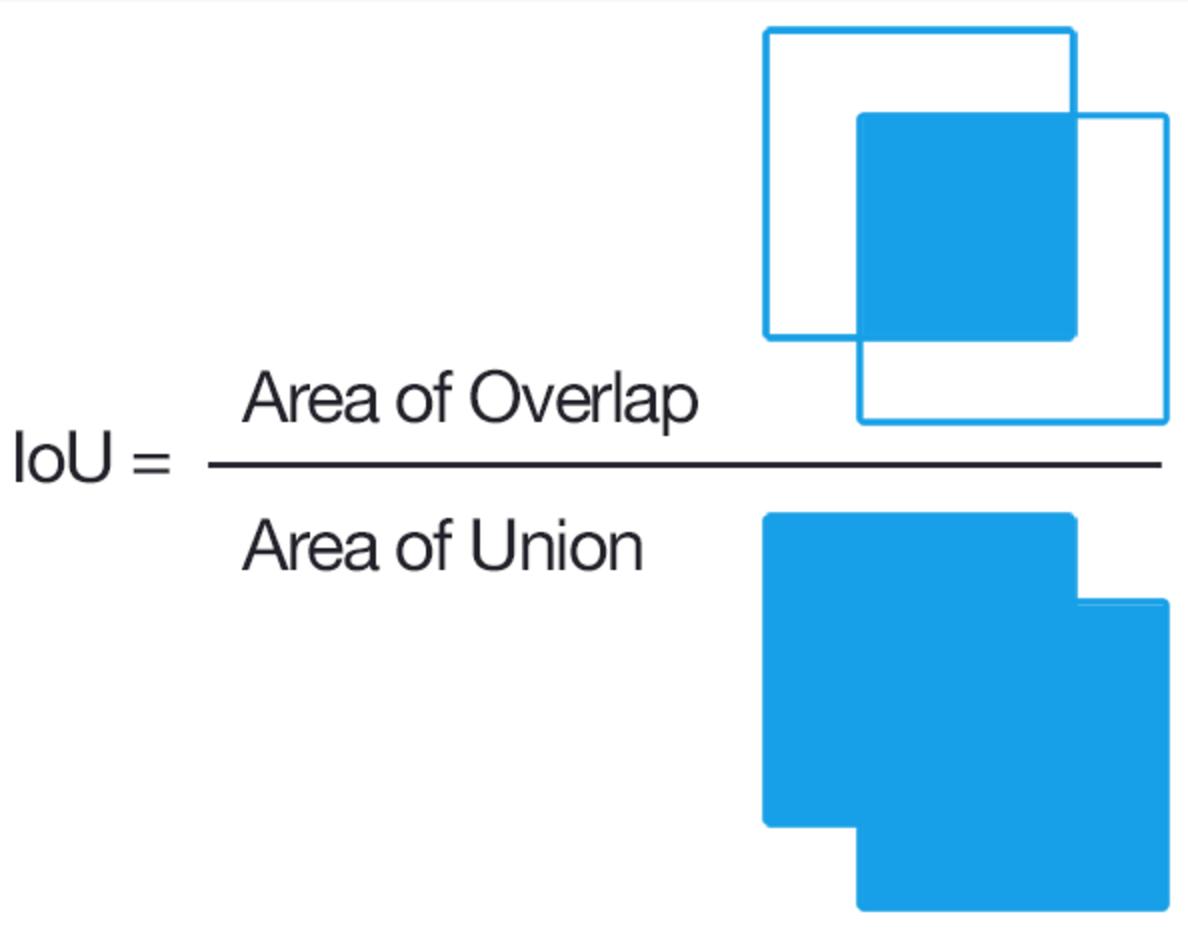
\includegraphics[width=0.5\textwidth]{iou.png}
\caption{Intersection over Union}
\end{figure}
Using the same instance we mentioned before, given the input image size is $224\times 224 \times 3$, feed the image to VGG-16, the output feature map size is $14\times 14\times 512$.Assume k=16.\[14\times 14\times 16\times 5=15680\] It is too expensive to train the RNN based on so many region proposals.So at training time, we sample B($B=256$) anchors as a minibatch, the minibatch contains less than B/2 positive anchors and the rest negatives.Before we sample regions, we should define negative and positive anchors.In this case ,we use Intersection over Union(IoU) to evaluate the similarity between anchorsand ground truth regions. IoU can be simple computed as the figure showing.

 Normally, a anchor is positive if$(i)$ it has an intersection over union(IoU) over 0.7 with all the ground truth region,or$(ii)$ ,it has the highest intersection over onion with a ground truth region.A anchors is negative if its IoU is lower than 0.3 with all the ground truth region. In training time,B region proposals were sampled uniformly  without replacement from negative bin and positive bin respectively.In testing time, anchors can be labeled as no ground truth provieded. So we use greedy non-maximum suppression(NMS) and confident score of regions to sample $B$ best region proposals.
 
 
After  sampling, we get a tensor of size $B\times 4$ which refer to a set of  region proposals with varying sizes.To communicate with next layer neural networks (Recurrent Neural Network), we have to convert the unfixed regions to fixed size features.In this case, the approach we are using is Bilinear Interpolation.Given a feature map $U$ of shape $C\times W'\times H'$ (in our instance is $512\times 14\times 14$) and sampled region proposals of shape $B\times 4$.By interpolating the feature map $U$ and refering to region proposals$(B\times 4)$, we generate a new feature map $V$ of shape $B\times C\times X\times Y$. \\
\begin{figure}[h]
\centering
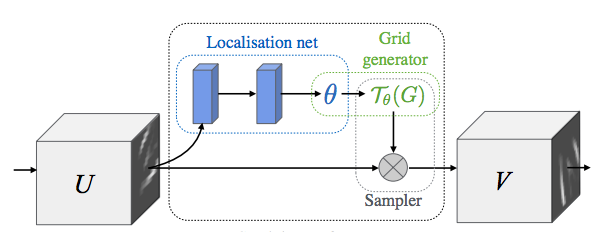
\includegraphics[width=0.8\textwidth]{transform.png}
\caption{Spatial Transformer}
\end{figure}


Concretely, before we compute a sampling grid $G$, we should project the region proposals onto feature map $U$.
Samping grid can be computed by:\\
\[ 
\left (
  \begin{tabular}{ccc}
  $x_i^s$ \\
  $y _i^s$
  \end{tabular}
\right ) =T_{\theta}(G_i)=A_{\theta}
\left (
  \begin{tabular}{ccc}
  $x_i^t$ \\
  $y _i^t$ \\
  1
  \end{tabular}
\right )=
\left [
  \begin{tabular}{ccc}
  $\theta_{11}$ &  $\theta_{12}$ &   $\theta_{13}$  \\
   $\theta_{21}$ &  $\theta_{22}$ &   $\theta_{23}$ 

  \end{tabular}
\right ] 
\left (
  \begin{tabular}{ccc}
  $x_i^t$ \\
  $y _i^t$ \\
  1
  \end{tabular}
\right )
\]
$$G=\{G_i\},G_i=(x_i^t,y_i^t)$$

Where $(x_i^s,y_i^s)$ are source coordinates of input feature map $U$, $(x_i^t,y_i^t)$ are target coordinates of output feature $V$.The two coordiantes $(x_i^s,y_i^s)$ and $(x_i^t,y_i^t)$ refer to the same pxiel, but in different tensors.To compute output tensor, we normally with a sampling kernel $k$.
\[V_i=\sum\limits_{m=1}^W\sum\limits_{n=1}^HU_{m,n}^c k(m-x_i^s)(n-y_i^s)\]
The height and width are normalized, so $-1<x_i^t,y_i^t<1$ and $-1<x_i^s,y_i^s<1$ . A bilinear sampler was used, which means $k$ refer to:
$$k(d)=max(0,1-|d|)$$\\
\begin{figure}[h]
\centering
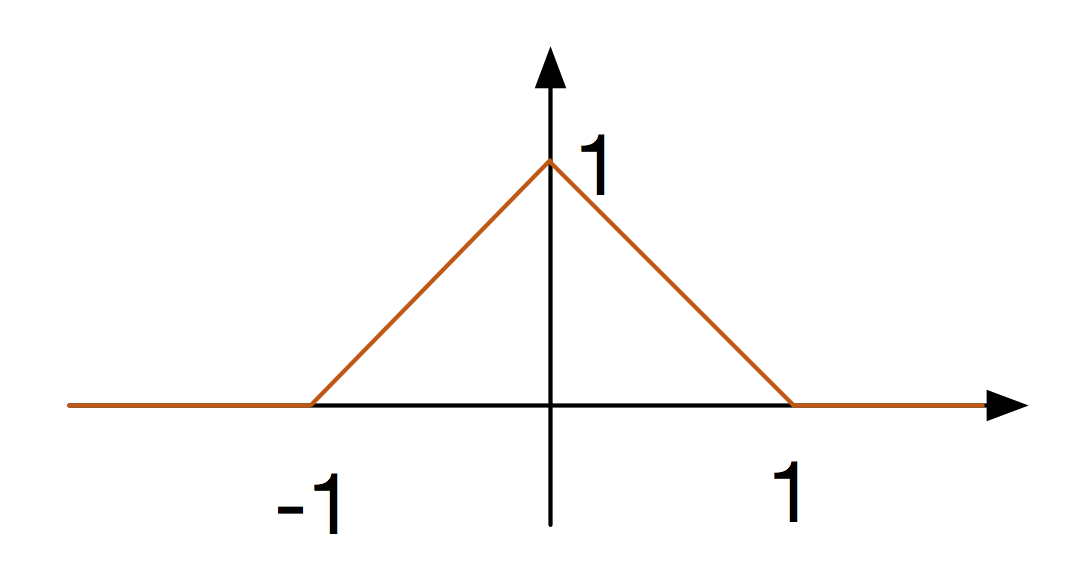
\includegraphics[width=0.8\textwidth]{bilinear2.png}
\caption{Bilinear Sampler}
\end{figure}

In summary, the Fully Convolutional Localization Network uses  shared  Conv features, The Conv features input to Region Proposal Network, then sampling B best region proposals and generate sampling grid.The same conv features input to bilinear sampler with sampling grid that give rise to  fixed-size region features.

\begin{figure}[h]
\centering
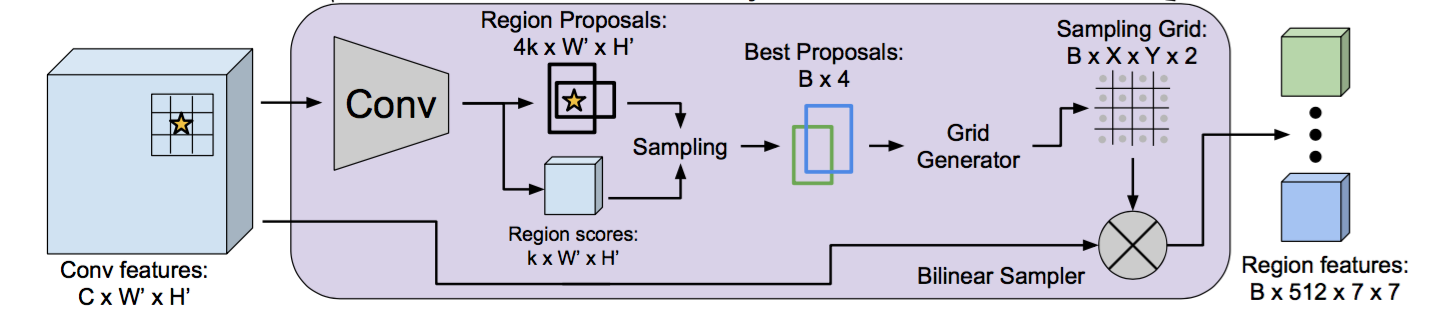
\includegraphics[width=0.9\textwidth]{rpn.png}
\caption{Region Proposal and Localization Network}
\end{figure}

The region features will input to a recognition neural network which is composed of  two fully connected  layers.The two fully connected layers using RELU as activation and regularized by dropout.Each region feature will convert to a vector then through the recognition network, after that it prodeces a 4096 dimension vector. 
\subsubsection{Recurrent Neural Network Languge Model}



\subsection{Web Interface}
\section{Implementation and Testing}
\section{Evaluation}
\section{Appraisal}
\section{Summary and Conclusion}
\section{Recommendation for Future Work}
\end{document}